\todo{Chainge for EWSM}

\begin{figure}[ht]
	\centering
	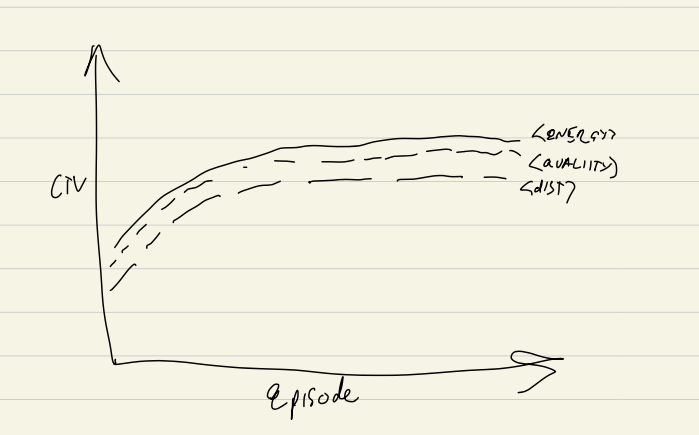
\includegraphics[width=0.8\linewidth]{5_ewsn_ctv}
	\captionsetup{labelfont=bf,singlelinecheck=on}
	\caption{System utility comparison to the system optimal in the optimal system}
	\label{fig:5_ewsn_ctv}
\end{figure}
\begin{figure}[ht]
	\centering
	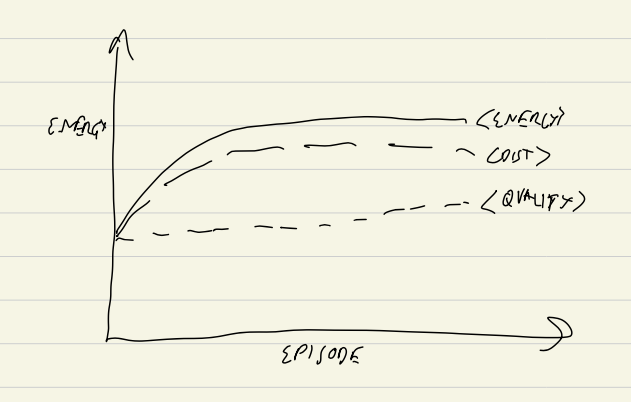
\includegraphics[width=0.8\linewidth]{5_ewsn_energy}
	\captionsetup{labelfont=bf,singlelinecheck=on}
	\caption{Energy available in the system as fraction of maximum}
	\label{fig:5_ewsn_energy}
\end{figure}
\begin{figure}[ht]
	\centering
	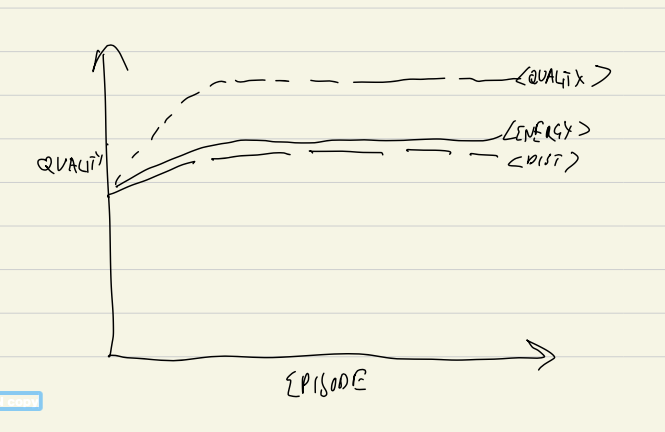
\includegraphics[width=0.8\linewidth]{5_ewsn_quality}
	\captionsetup{labelfont=bf,singlelinecheck=on}
	\caption{Quality compared to system optimal}
	\label{fig:5_ewsn_quality}
\end{figure}

\begin{figure}[ht]
	\centering
	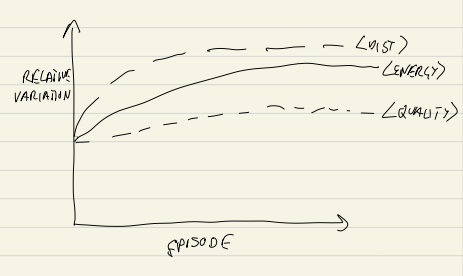
\includegraphics[width=0.8\linewidth]{5_ewsn_relative_variation}
	\captionsetup{labelfont=bf,singlelinecheck=on}
	\caption{Relative variability of energies}
	\label{fig:5_ewsn_relative_variation}
\end{figure}
